%=========================================================================
% sec-xpc
%=========================================================================

\section{Explicit-Parallel-Call Architectures}
\label{sec-xpc}

In software, XPC applications use a highly productive parallel
programming library allowing users to cleanly \emph{expose} varying forms
of amorphous data parallelism as fine-grain parallel tasks. Tasks are
exposed to hardware as parallel function calls via a unifying XPC
ISA. Parallel tasks can be \emph{executed} on a heterogeneous mix of
general-purpose and data-parallel accelerator tiles that implement the
XPC ISA (i.e., XPC tiles). The parallel tasks exposed in software are
adaptively \emph{scheduled} onto the hardware tiles they are best suited
for via a software runtime with hardware support for storing and
distributing tasks.

\subsection{Exposing Fine-Grain Parallel Tasks}

Traditional parallel programming frameworks are \emph{platform-centric},
meaning the user must write code for a specific platform (e.g.,
OpenMP~\cite{openmp3-spec2008} and POSIX threads for general-purpose
multicores, CUDA~\cite{nvidia-kepler-wpaper2012} for GPGPUs). Although
the OpenCL~\cite{opencl1-spec2011} framework was designed for
heterogeneous architectures, thus is more platform agnostic, parallelism
is exposed at a coarse granularity and there is no support for nested
parallelism, limiting the types of algorithms that can be used to
implement applications.
The XPC programming framework is also platform agnostic, but exposes
parallelism at a finer granularity and provides support for nested
parallelism. This \emph{algorithm-centric} framework allows users to
focus on exploring different algorithms for implementing a given
algorithm (e.g., recursive, iterative, frontier-based, speculative,
etc.) and flexibly evaluate the tradeoffs of mapping different algorithms
to different XPC tiles.
The XPC programming framework offers multiple parallel primitives to make
encoding amorphous data parallelism easier. Figure~\ref{fig-xpc-api}
shows a preliminary sketch of how the XPC library could be used to
parallelize an example application. The \TT{spawn} primitive is used to
recursively generate tasks in a divide-and-conquer approach similar to
Intel Cilk++~\cite{cilk-spec2010}. The \TT{parallel\_for} primitive is
used to parallelize iterations/tasks of a loop. The \TT{atomic\_for}
primitive is similar to \TT{parallel\_for} except that it guarantees
iterations/tasks are processed atomically with respect to other
iterations/tasks. This primitive is ideal for amorphous data parallel
applications with highly conflicting tasks. We take advantage of modern
C++11 lambda functions to achieve a clean and convenient method for
defining tasks. Variables used in the lambda are automatically captured
by reference, and the API handles passing in the appropriate index as an
argument to the function.

\begin{figure}
  \begin{minipage}[b]{0.44\tw}
    %=========================================================================
% fig-xpc-api.tex
%=========================================================================

%\begin{figure*}

  \cbxsetfontsize{8pt}
  \begin{subfigure}{\tw}
  \begin{Verbatim}[gobble=6]
    void bfs( Node nodes[] ) {
      xpc::spawn( start, func = [&] (int idx) {

        Node my_node = node[idx];

        for ( i = 0; i < my_node.num_neigh; i++ ) {

          Node neighbor = my_node.neighbors[idx];

          if ( my_node.dist + 1 < neighbor.dist ) {
            neighbor.dist = my_node.dist + 1;
            xpc::spawn( neighbor.idx, func );
          }
        }});}
  \end{Verbatim}
  \end{subfigure}

  \caption{\BF{Example Code Using XPC Programming API --} Preliminary
    ideas for how the XPC programming API could be used to parallelize
    amorphous data parallel applications. The \TT{spawn} primitive is
    used to parallelize the breadth-first search application using a
    divide-and-conquer algorithm.}
  \label{fig-xpc-api}

%\end{figure*}

  \end{minipage}%
  \hfill%
  \begin{minipage}[b]{0.54\tw}
    %=========================================================================
% fig-xpc-isa.tex
%=========================================================================

%\begin{figure}

  \centering
  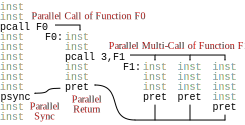
\includegraphics[width=\tw]{xpc-isa.svg.pdf}

  \caption{\textbf{XPC Instruction Set Overview --} Parallel calls and
    parallel multi-calls (\TT{pcall}) encode opportunities for parallel
    execution, which the architecture may (or may not) choose to exploit.
    Parallel synchronization points (\TT{psync}) require all child
    parallel calls to complete before continuing. All parallel returns
    (\TT{pret}) are implicitly synchronization points.}

  \label{fig-xpc-isa}

%\end{figure}


  \end{minipage}
\end{figure}

The XPC ISA extends a traditional RISC ISA with three new instructions: a
parallel function call instruction (\TT{pcall}), a parallel function
return instruction (\TT{pret}), and a parallel synchronization
instruction (\TT{psync}). A parallel function call enables the software
to inform the hardware that it is acceptable to execute the callee in
parallel with the caller, but critically, parallel execution is \emph{not
  required}. A serial execution of any \TT{pcall} should always be an
acceptable execution. As illustrated in Figure~\ref{fig-xpc-isa},
\TT{pcall}s can be nested to arbitrary depths, and recursive \TT{pcall}s
are also allowed. A \TT{psync} acts as a synchronization point (i.e.,
barrier) and waits for all child \TT{pcall}s to finish execution. For a
serial execution a \TT{psync} is essentially a \TT{nop}. A \TT{pret}
returns from a \TT{pcall} and also acts as an implicit synchronization
point. A particularly novel feature of the XPC ISA is the capability for
parallel multi-calls. A parallel multi-call enables the software to
inform the hardware that the given function should be executed $n$ times
where $n$ can be either specified at compile time or run time. While it
is certainly possible to achieve the same effect by using a basic
\TT{pcall} within a loop, a parallel multi-call enables very efficient
execution on certain XPC tiles.

\subsection{Executing Fine-Grain Parallel Tasks}

The underlying XPC microarchitecture is a heterogeneous mix of XPC tiles
that are specialized for exploiting a broad range of amorphous data
parallelism.

\textbf{XPC Tightly-Coupled Lanes (TCL) --} The TCL tile is a
data-parallel accelerator specialized for conventional data parallelism. A
simple in-order, single-issue control processor is tightly coupled with a set
of computation lanes. Instruction fetch and decode are
amortized by the control processor and an issue unit schedules a group of
threads that execute in lock-step on the tightly-coupled lanes. Control
irregularity can cause divergence between threads, serializing execution
of both paths of the branch. Memory accesses are dynamically coalesced by
a memory unit by comparing the addresses generated across the
lanes. Unlike GPGPUs, the TCL tile focuses on exploiting intra-warp
parallelism instead of relying on extreme temporal multithreading to
exploit inter-warp parallelism, dramatically reducing the area
overhead. Due to its lightweight, embedded design, the TCL tile is a
natural fit for XPC's heterogeneous microarchitecture. The TCL tile is
inspired by our previous work in accelerating conventional data parallel
applications on GPGPUs by exploiting value
structure~\cite{kim-simt-vstruct-isca2013}. Similar techniques can be
used to eliminate redundant computation on the TCL tile.
% to further improve the performance and energy efficiency of conventional
% data parallel tasks.

Although the TCL tile will achieve high performance and energy efficiency
by amortizing the front-end and memory accesses as well as exploiting
value structure for conventional data parallel tasks, it will struggle
with the serialization caused by control and memory-access irregularity
in more amorphous data parallel tasks.

\textbf{XPC Loosely-Coupled Lanes (LCL) --} The LCL tile is an
accelerator specialized for more irregular amorphous data
parallelism. The key difference between the TCL and LCL tiles is that the
LCL tile decouples control flow between lanes without significant
overheads. This is achieved by using per-lane instruction buffers which are
populated by the control processor and can contain different sections of
code for each lane to execute. The control processor still amortizes
instruction fetch and a lane management unit distributes tasks across the
lanes. Each LCL lane is more lightweight than the TCL counterpart as it
shares expensive long-latency functional units between all lanes and the
control processor. As a result, more LCL lanes can be employed than TCL
lanes for roughly the same cost. The LCL design is inspired by previous
work in my research group on accelerating loop patterns in
hardware~\cite{srinath-xloops-micro2014}.

The LCL tile can be used a reasonable middle-ground for accelerating
amorphous data parallelism before resorting to a general-purpose tile
because of its higher tolerance for control irregularity. However, the
LCL tile is still better suited for simpler tasks on the lanes and can
suffer from high memory-access irregularity.

\textbf{XPC Cooperative Multicore (CMC) --} The CMC tile is a
general-purpose multicore processor designed to be used for highly
irregular amorphous data parallel applications that cannot be efficiently
accelerated on other XPC tiles. A grid of discrete cores are connected by
a crossbar to facilitate rapid inter-core communication. Each CMC core,
albeit relatively simple, is akin to a stripped-down control processor in
a TCL/LCL tile, making it capable of handling high control and
memory-access irregularity with acceptable performance. The tradeoff is
that CMC is the least energy efficient tile of the three XPC tiles for
applications which exhibit more regular amorphous data parallelism. They
key difference between the CMC tile and a traditional multicore is that
the CMC tile uses hardware acceleration for scheduling fine-grain
parallel tasks as discussed below.

The CMC tile could function as a default tile for the profiling phase
when statistics are collected to determine if an accelerator tile would be
more suitable, in addition to being the optimal tile for highly irregular
amorphous data parallel tasks which cannot fully utilize the amortization
offered by the TCL or LCL tiles.

\subsection{Scheduling Fine-Grain Parallel Tasks}

\begin{figure}
  \begin{minipage}[b]{0.53\tw}
    %=========================================================================
% fig-xpc-task-cache.tex
%=========================================================================

%\begin{figure}

  \centering
  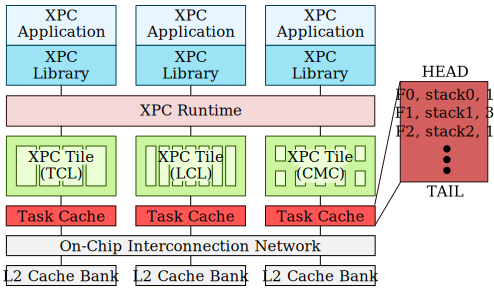
\includegraphics[width=\tw]{task-cache.svg.pdf}

  \caption{\textbf{Task Cache Diagram --} Per-core task caches store
    generated tasks in hardware as a triplet of a function pointer, a
    stack pointer, and the number of calls for the task.}

  \label{fig-xpc-task-cache}

%\end{figure}


  \end{minipage}%
  \hfill%
  \begin{minipage}[b]{0.45\tw}
    %=========================================================================
% fig-xpc-task-network.tex
%=========================================================================

%\begin{figure}

  \centering
  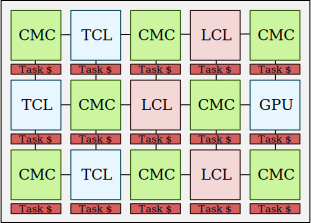
\includegraphics[width=\tw]{task-network.svg.pdf}

  \caption{\textbf{Task Distribution Network Diagram --} Network
    connecting task caches for rapid distribution of tasks across
    heterogeneous XPC tiles based on meta-data describing task affinity
    with given tile.}

  \label{fig-xpc-task-network}

%\end{figure}


  \end{minipage}
\end{figure}

The fine-grain parallel tasks exposed in software are mapped to the XPC
tiles in hardware through a software runtime that adaptively schedules
tasks onto the best suited tiles. This process can be accelerated in
hardware with a \emph{task cache} and \emph{task distribution network}.

One way for the software runtime to manage exposed tasks is to use a
cactus stack in memory~\cite{frigo-hyperobjects-spaa2009} that keeps
track of separate views of the stack whenever opportunities for parallel
tasks are generated. The runtime associates each task with a function
pointer, a pointer to the corresponding view of the stack in
the cactus stack, and the number of calls required. This meta-data is
stored in a per-tile task queue from which other tiles can steal tasks
through the runtime. A critical component to the task stealing in the
context of a heterogeneous architecture is determining key heuristics
for accurately predicting the optimal tile for executing a task. An
initial idea is to collect statistics on control and memory-access
irregularity to proxy performance and energy efficiency. Higher
irregularity would suggest the task is better suited for more
general-purpose tiles, whereas highly regular tasks would be better
suited for data-parallel accelerator tiles.

The runtime normally generates and distributes tasks through memory, but
hardware acceleration can be used to streamline these
processes. Figure~\ref{fig-xpc-task-cache} shows a per-tile \emph{task
  cache} that exploits intra-tile task locality by storing entries of the
task queue in a hardware cache to avoid memory accesses. This is based on
the observation that each thread or tile will almost always need to
access its own task queue whenever it is ready to execute a new
task. Furthermore, Figure~\ref{fig-xpc-task-network} shows a \emph{task
  distribution network} connecting task caches to facilitate rapid
distribution of tasks to tiles attempting to steal tasks. The runtime
triggers a broadcast of task steal requests if the tile it is running on
is idle. For scalability, the request is only broadcasted to the tile's
direct neighbors. The network also communicates meta-data with each
request describing the type of task for which it is best suited, which
can considered along with collected heuristics to determine whether or
not a tile should allow task stealing. These hardware techniques for
storing and distributing tasks is inspired by our previous work in task
distribution for amorphous data parallel applications on
GPGPUs~\cite{kim-hwwl-micro2014}.
